\textbf{Étape 1 : Chargement de la base dans eXist-db}

\begin{flushleft}
- Lancer eXist-db et ouvrir le localhost \\
- Se rendre dans l'onglet « Package Manager » \\
- Faire glisser le fichier « .xar » dans la « DROPZONE » \\
- Pour supprimer l'application ThEMA il suffit de cliquer sur l'icône poubelle dans la liste des packages installés \\ 
\end{flushleft}

\begin{figure}[H]
	\centering
	\fbox{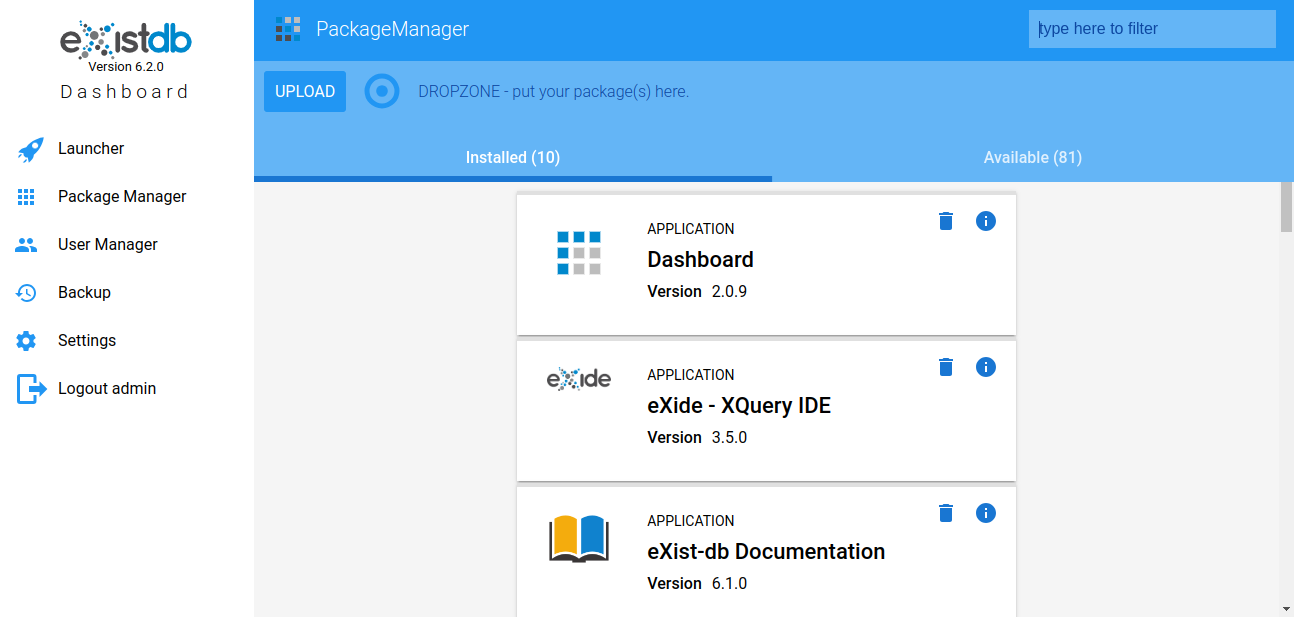
\includegraphics[width=0.8\linewidth]{images/existdbpackagemanager.png}}
	\caption{Page « Package Manager » de eXist-db}
\end{figure}

\textbf{Étape 2 : Création des groupes de sécurité} 

\begin{flushleft}
	- Faire clic droit sur l'icône eXist-db \\
	- Cliquer sur Open Java Admin Client \\ 
	- Créer un nom d'utilisateur, un mot de passe et mettre dans les favoris « localhost » \\
	- Ouvrir « Outils » puis « Éditer les utilisateurs » \\
	- Créer quatre groupes « indexer », « editor », « project-contributor » et « project-engineer » \\
	- Par défaut, eXist-db nous identifiera comme admin \\
\end{flushleft}	

\begin{figure}[H]
	\centering
	\fbox{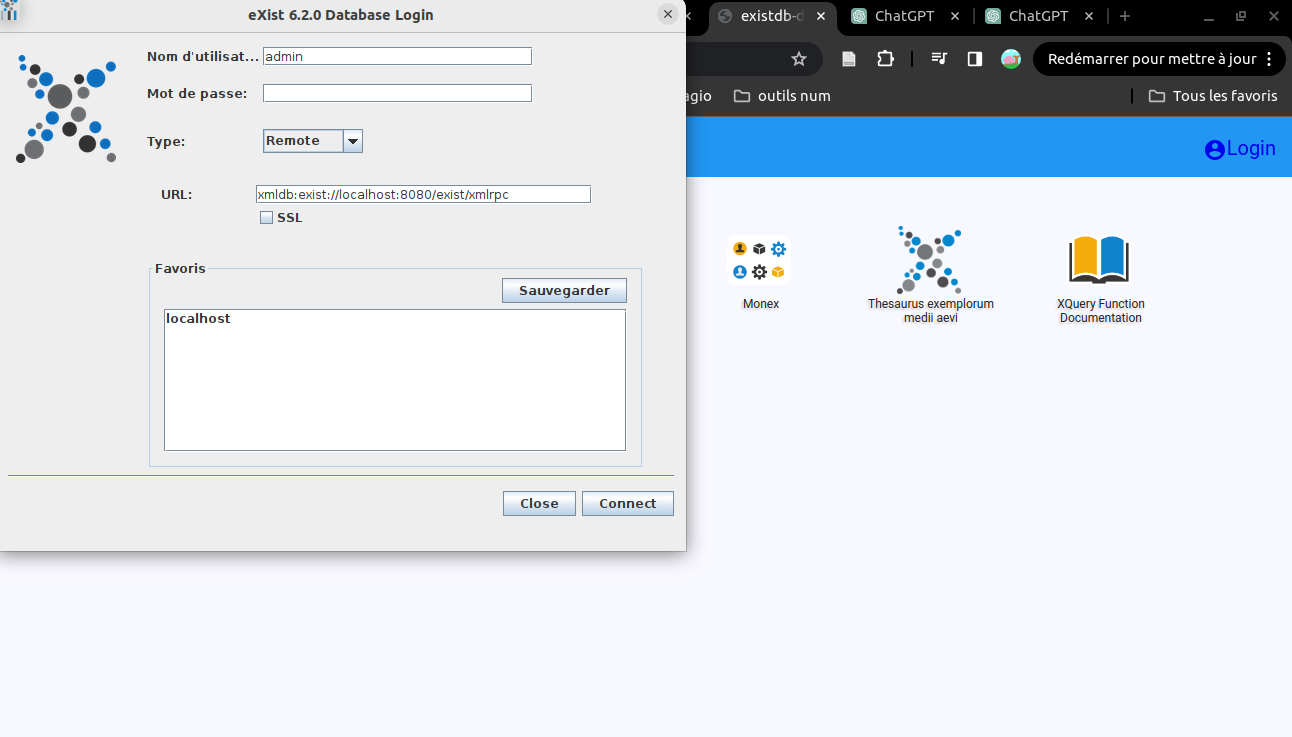
\includegraphics[width=0.6\linewidth]{images/adminexist.png}}
	\caption{Modification dans l'Admin client n°1}
\end{figure}
	
\begin{flushleft}	
	- Aller dans « apps », « thema », « modules » \\
	- Ouvrir « dbfunction » en cliquant sur « Editer les propriétaires » \\
	- Cocher « SetUID » et « SetGID » \\ 
	- Ouvrir « user.xql », cocher toutes les cases de la colonne « Execute » et passer du groub « dba » à « thema » \\

\end{flushleft}	
	
\begin{figure}[H]
	\centering
	\fbox{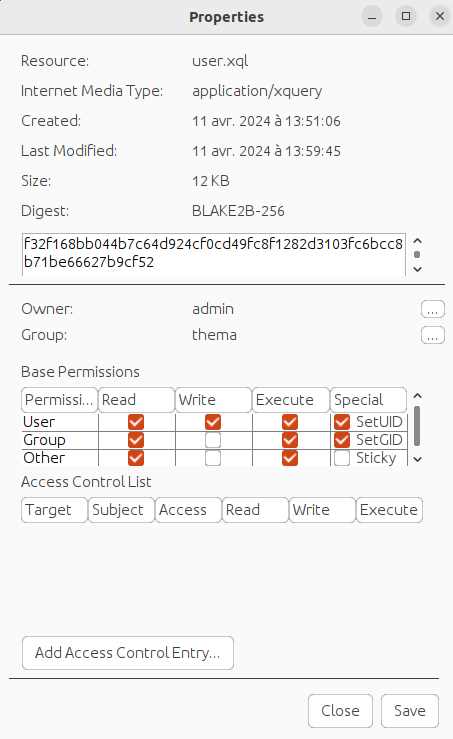
\includegraphics[width=0.3\linewidth]{images/dba.png}}
	\caption{Modification dans l'Admin client n°2}
\end{figure}
	
\textbf{Étape 3 : Compléter la base} 

\begin{flushleft}	
	- Aller dans eXide \\ 
	- Aller dans « File » puis « Manage » \\
	- Se rendre à l'endroit de l'arborescence et cliquer sur « Upload Files » \\ 
	- Faire glisser les données et appuyer sur « done » quand le chargement est terminé \\
	- Les dossiers et fichiers à ajouter sont ceux présents dans la copie de la base mais qui ne sont pas dans eXist-db \\
	- Ne pas mettre trop de fichiers en même temps et bien attendre que la roue dentée arrête de tourner \\
	- vérifier que les documents sont bien implémentés \\
	
	 - Se rendre dans « apps », « thema » \\
	 - Lancer les fichiers « .xconf » en appuyant sur « Eval » \\
	 - En cas d'ajouts de données, il sera nécessaire de lancer à nouveau l'évaluation \\ 
	 - Modifier « var base URL = » avec : « 'https://localhost:8080/exist/apps/thema/' » \\
\end{flushleft}
	
\begin{figure}[H]
	\centering
	\fbox{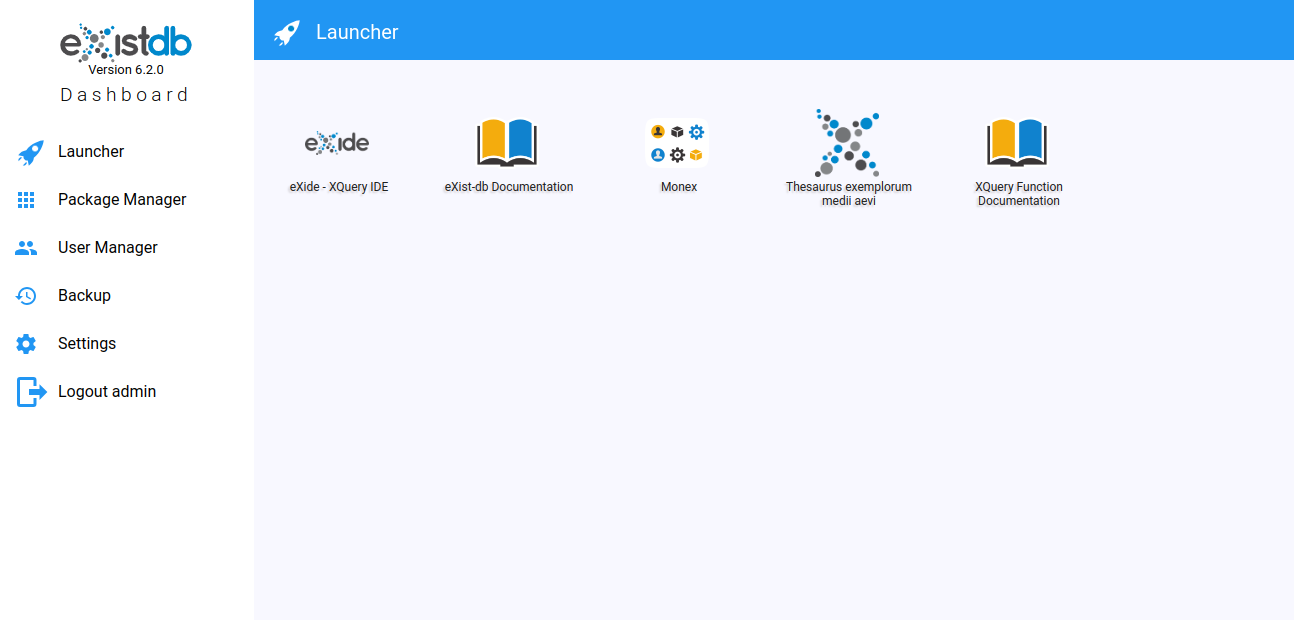
\includegraphics[width=0.8\linewidth]{images/exideexistdb.png}}
	\caption{Page d'accueil d'eXist-db}
\end{figure}

\begin{figure}[H]
	\centering
	\fbox{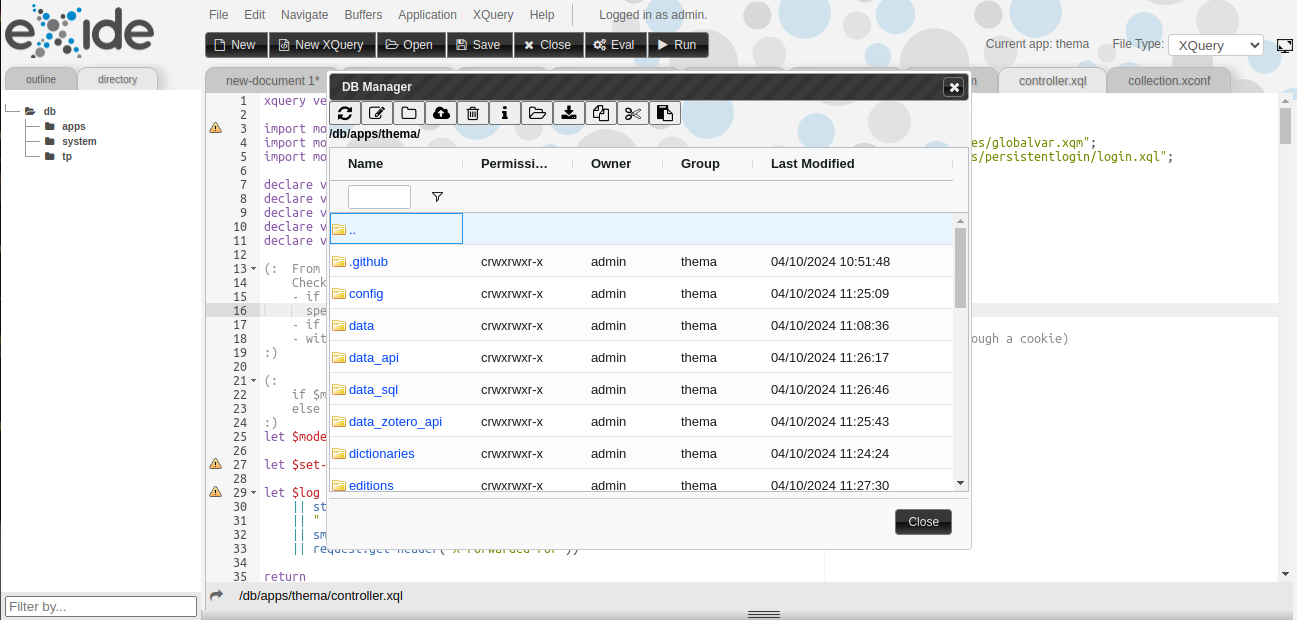
\includegraphics[width=0.8\linewidth]{images/implementationexide.png}}
	\caption{Page d'accueil « Upload Files »}
\end{figure}
	
\textbf{Étape 4 : Lancer et éteindre la base de données} 
	
\begin{flushleft}
	- Se rendre dans le « Launcher » de eXist-db \\
	- Cliquer sur « ThEMA » \\
	- Essayer toutes les fonctionnalités pour vérifier s'il n'y a pas de bogue \\
	
	- Cliquer sur l'icône eXist-db et cliquer sur « Stop server » \\
	- Cliquer sur « Quit »\\
	- Si cette manipulation n'est pas réalisée, il y a un risque d'altération des données et de la structure de la base \\
	
\end{flushleft}
	
\textbf{Étape 5 : Création d'un back-up} 
	 
\begin{flushleft}
	 - Chercher l'endroit où est installé eXist-db sur l'ordinateur \\
	 - Ouvrir le fichier « conf.xml » et remplacer « true » par « false » dans « posix-chown-restricted » \\
	 - Ajouter dans les balises « <scheduler> </scheduler> », le code suivant : \\
	 
\end{flushleft}

\begin{lstlisting}[breaklines=true]
	 	<job type="system" class="org.exist.storage.ConsistencyCheckTask"  cron-trigger="0 10 2 * * ?">
	 	<parameter name="output-dir" value="backup"/>
	 	<parameter name="zip" value="yes"/>
	 	<parameter name="backup" value="yes"/>
	 	<parameter name="incremental" value="no"/>
	 	<parameter name="incremental-check" value="no"/>
	 	</job>
\end{lstlisting}

\begin{flushleft}
	 - Aller dans « Fenêtre », « Afficher la vue », « Explorateur de sources de données » \\
	 - Se connecter à eXist-db localhost \\
\end{flushleft}

\begin{figure}[H]
	\centering
	\fbox{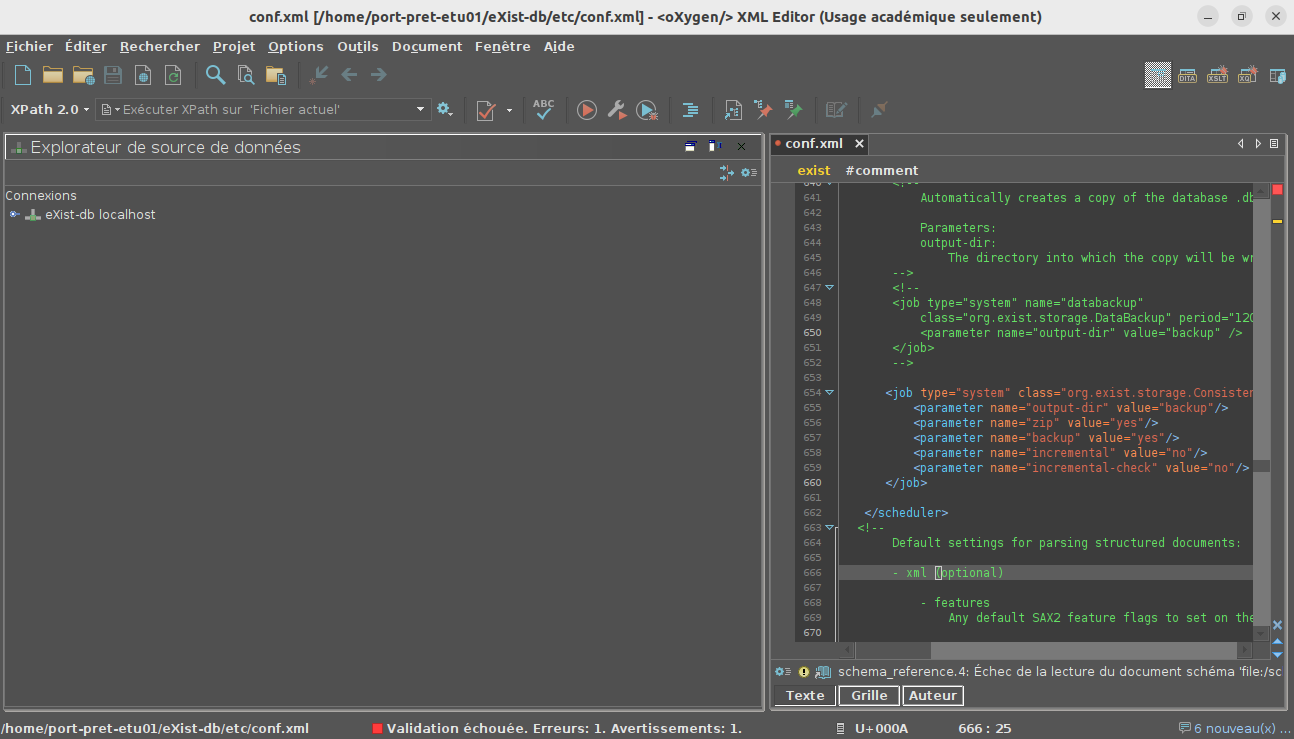
\includegraphics[width=0.8\linewidth]{images/oxygen.png}}
	\caption{Utilisation de Oxygen pour coder en lien avec eXist-db}
\end{figure}